\documentclass[11pt]{article}
\usepackage{geometry}
\geometry{a4paper}
%\geometry{landscape}
\usepackage[parfill]{parskip}    % Activate to begin paragraphs with an empty line rather than an indent
\usepackage{graphicx}
\usepackage{amssymb}
\usepackage{epstopdf}
\usepackage{fancyhdr}
\usepackage{fullpage}
\usepackage{appendix}
\usepackage{newclude}
\usepackage{datetime}
\usepackage{hyperref}
\usepackage{color}
\usepackage{multind}
\usepackage{microtype}

\makeindex{pve}
\newcommand{\pve}[1]{\index{pve}{#1}#1}
\newcommand{\pvelist}[1]{ \begin{footnotesize} PvE: #1 \end{footnotesize} \\ }

\makeindex{drupalpath}
\newcommand{\drupalpath}[1]{\index{drupalpath}{#1}\texttt{dimpact.nl/#1}}



\hypersetup{
    colorlinks,
    citecolor=black,
    filecolor=black,
    linkcolor=black,
    urlcolor=black
}

\DeclareGraphicsRule{.tif}{png}{.png}{`convert #1 `dirname #1`/`basename #1 .tif`.png}

\newcommand{\seeone}[1]{ (zie \ref{#1} p.\pageref{#1})}
\newcommand{\seetwo}[2]{ (zie \ref{#1} p.\pageref{#1},  \ref{#2} p.\pageref{#2})}

\pagestyle{fancy}
\fancyhead{}
\fancyfoot{}
\fancyfoot[R]{\thepage}

\setcounter{secnumdepth}{4}
\setcounter{tocdepth}{2}

\makeatletter
\renewcommand\paragraph{%
   \@startsection{paragraph}{4}{0mm}%
      {-\baselineskip}%
      {.5\baselineskip}%
      {\normalfont\normalsize\bfseries}}
\makeatother

\newcommand{\customer}{Dimpact }
\newcommand{\thecustomer}{\customer }
\newcommand{\customerdomain}{dimpact}
\newcommand{\customerdomainuc}{Dimpact.nl}

\title{Handleiding \customerdomainuc}
\author{Mike Hens \\ Maurits Lawende \\ Patrick Kraaij \\ Maarten Hartman}
\date{}

\begin{document}
\maketitle
\begin{center}
%
\includegraphics{img/logo.jpg}

Laatst bijgewerkt: \\ \ddmmyyyydate \today
\end{center}
\pagebreak

\renewcommand*\contentsname{Inhoudsopgave}
\tableofcontents
\pagebreak

%\subsection{Workbench}\label{workbench}
De workbench biedt een handig overzicht voor (eind)redacteuren. Via de workbench kun je bijvoorbeeld makkelijk bekijken welke inhoud recentelijk is aangemaakt of welke inhoud nog beoordeeld moet worden.

\subsubsection{Workbench overview}\label{workbenchoverview}
De onderstaande afbeelding toont de Workbench. 
\bigskip

\begin{center}
	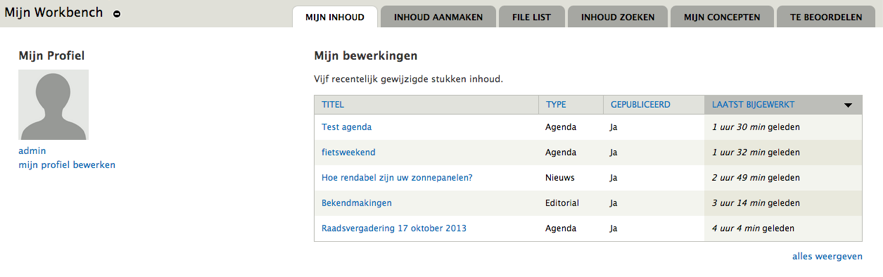
\includegraphics[width=\textwidth]{img/workbench.png}
\end{center}

\textbf{Mijn inhoud:} toont de inhoud welke recentelijk is bewerkt door de gebruiker.

\textbf{Inhoud toevoegen:} link naar de pagina \emph{Inhoud toevoegen}.

\textbf{File list:} toont alle bestanden welke recentelijk zijn toegevoegd.

\textbf{Inhoud zoeken:} link naar de pagina \emph{Inhoud zoeken}, hier kun je gemakkelijk met behulp van filters op inhoud zoeken.

\textbf{Mijn concepten:} toont alle concepten aangemaakt door de gebruiker.

\textbf{Te beoordelen:} toont alle content items welke nog goedgekeurd moeten worden door de eindredacteur.

\subsubsection{Workbench workflow}\label{workbenchworkflow}

De workflow binnen de workbench gaat als volgt. Een redacteur voert nieuwe content op als \emph{concept}. Zolang het een concept blijft zal deze terug te vinden zijn onder de tab \emph{Mijn concepten}. Dit item zal dan niet aan de voorkant te lezen zijn. De redacteur kan dan kiezen om het ter beoordeling aan te bieden. Het item zal dan verschijnen onder de tab \emph{Te beoordelen} van een gebruiker met de rol \emph{eindredacteur}. De eindredacteur kan dan kiezen om het item terug te zetten naar concept of om het te publiceren. 

Bij het bewerken van bestaande content geldt dezelfde flow. Van het bestaande item zal dan een nieuw concept gemaakt worden, wat door de redacteur ter beoordeling aangeboden kan worden. Om daarna door een eindredacteur te publiceren of terug te zetten naar concept.
\subsection{Social media}

Ter ondersteuning van het delen op social media wordt voorzien in de volgende zaken:
\begin{itemize}
\item Share buttons
\item Mogelijkheid om widgets in HTML code te plaatsen
\item RSS feeds
\end{itemize}

\subsubsection{Share buttons}

De share buttons geven de mogelijkheid om de pagina te delen op de verschillende sociale media. Hierin kunnen de volgende buttons worden ingesteld:
\begin{itemize}
\item Facebook
\item Google+
\item LinkedIn
\item Twitter
\item Delen op Facebook (widget)
\item Twitteren (widget)
\end{itemize}

Bij oplevering van de standaarddistributie worden de specifieke share links aangezet. De widgets worden niet ingesteld. Deze kunnen bij implementatie van de gemeentesites makkelijk worden aangezet. De theming zal wel geschikt worden gemaakt voor het grotere formaat van deze widgets.

Buttons worden op alle nodetypes toegevoegd die een detailpagina hebben.

Per subsite wordt instelbaar of de share buttons direct zichtbaar zijn of onder een overlay komen. In het laatste geval is een enkele "delen" link beschikbaar waarmee de overlay geopend kan worden. Voor deze instelling wordt een custom \emph{dominion functie} aangemaakt met de systeemnaam \texttt{sharelink}. In het theme kan dan gebruik gemaakt worden van de functie \texttt{dominion\_has\_function} om te bepalen of de overlay gebruikt moet worden.

\subsubsection{Widgets in HTML-code}

Eindredacteuren krijgen de mogelijkheid om zelf HTML widgets te plaatsen in de body tekst\seeone{invoerformaten}.

\subsubsection{Externe RSS-feeds}

Via de \usemodule{views} module i.c.m. de \usemodule{views\_rss} module worden RSS feeds ingesteld. De volgende feeds worden aangemaakt:
\begin{enumerate}
\item Laatste nieuwsberichten
\item Actuele evenementen
\item Laatste bekendmakingen
\item Laatst gewijzigde pagina's
\end{enumerate}
De views worden gesorteerd op publicatiedatum (1 t/m 3) of datum laatst gewijzigd (4). De RSS feed laat altijd 20 items zien.

Nieuwe RSS feeds kunnen niet door de gemeente aangemaakt worden.



\section{Content editing}\label{contentedit}

\subsection{Rechten en rollen}

\pvelist{ \pve{2.8.1}, \pve{2.8.2}, \pve{2.8.3}, \pve{2.8.5} }

Het CMS beschikt over de mogelijkheid om rollen toe te wijzen aan gebruikers toegangsrechten in te stellen per gebruikersrol. De volgende rollen zijn gedefini\"{e}erd:
\begin{itemize}
\item Eindredacteur \\ Kan alle inhoud beheren
\item Redacteur \\ Kan inhoud beheren op toegewezen onderdelen van de website. Een eindredacteur kan wel inhoud van een redacteur publiceren op andere delen van de website.
\item Administrator (webmaster) \\ Kan alle inhoud beheren.
\end{itemize}
Opties die voor een gebruiker niet beschikbaar zijn (vanwege de ingestelde permissies) zijn niet zichtbaar.

Redacteuren dienen aan een deel van de website (subsite) te worden gekoppeld. Dit kan een webmaster of eindredacteur doen. Hiervoor moet het gebruikersaccount worden bewerkt (de gebruiker kan worden opgezocht via \emph{Personen} in de werkbalk).  Bij het bewerken van een account is een lijst van subsites beschikbaar. De redacteur kan content publiceren op de subsites die daar worden aangevinkt.

\subsection{Dashboard}\label{dashboard}
\pvelist { \pve{2.11.2} }
Elke redacteur heeft toegang tot het dashboard. Het dashboard kan worden gebruikt om inhoud op te zoeken, en bevat lijsten van recente bewerkingen, goed te keuren inhoud etc. Als dashboard wordt de \emph{Workbench} module gebruikt. Deze is beschikbaar in de werkbalk onder \emph{Mijn workbench}.

De pagina opent standaard met de tab \emph{Mijn inhoud}. Op deze pagina zijn korte lijsten beschikbaar met de laatste bewerkingen en de laatste inhoud. Tevens is er een eenvoudige zoekbox beschikbaar waarmee gezocht kan worden binnen alle inhoud. Naast deze zoekfunctie kan ook gebruik gemaakt worden van de uitgebreidere zoekfunctie in \emph{Mijn inhoud}\seeone{alleinhoud}.

\subsubsection{Mijn inhoud}\label{mijninhoud}

Deze pagina laat de laatste bewerkingen zien die gemaakt zijn door de ingelogde gebruiker. Daaronder staat een lijst met de laatst toegevoegde inhoud van alle gebruikers.

\subsubsection{Alle inhoud}\label{alleinhoud}
\pvelist{ \pve{2.3.8}, \pve{2.11.1}, \pve{2.11.3}, \pve{2.11.4}, \pve{2.11.5}, \pve{2.11.6}, \pve{2.11.7}, \pve{2.11.8}, \pve{2.11.9}, \pve{2.11.10}, \pve{2.11.13}, \pve{2.11.14}, \pve{2.11.15}, \pve{2.11.16} }
In het dashboard kan alle inhoud worden doorzocht. Ga hiervoor naar \emph{Mijn Workbench} $\Rightarrow$ \emph{Inhoud zoeken}, of ga direct naar \drupalpath{admin/workbench/all-content}. De lijst kan verder worden gefilterd op bijvoorbeeld alleen ongepubliceerde inhoud. Vul daarvoor de velden in en klik op \emph{Toepassen}.
\begin{center}
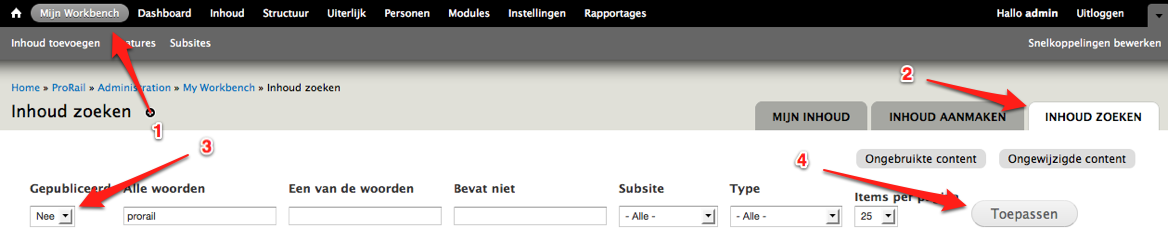
\includegraphics[width=\textwidth]{img/ongepubliceerdeinhoud.png}
\end{center}
De volgende filtering is mogelijk:
\begin{itemize}
\item Gepubliceerd \\
Hiermee kan worden gefilterd op alleen wel of niet gepubliceerde inhoud.
\item Alle woorden \\
Alle opgegeven woorden moeten voorkomen in de bodytekst. Woorden worden ook gevonden wanneer een deel van het woord is gegeven.
\item Een van de woorden \\
Minimaal \'{e}\'{e}n van de woorden moet voorkomen in de bodytekst.
\item Bevat niet \\
Deze tekst mag niet voorkomen in de bodytekst.
\item Subsite \\
Limiteer de resultaten tot een enkele subsite (doelgroep / project).
\item Type \\
Limiteer de resultaten tot een specifiek inhoudstype.
\end{itemize}
Daarnaast kan het aantal items per pagina worden opgegeven. Na het zoeken blijft de filtering staan en is het mogelijk om de opdracht te verfijnen door de filtering aan te passen. De sortering van de zoekresultaten kan worden aangepast door op de koppen van de tabel te klikken.

In het zoekresultaat verwijst de titel naar de pagina zelf. Daarnaast is er een bewerk-link beschikbaar. Na het bewerken van de node keert men terug naar de lijst met zoekresultaten. Bij het bezoeken van de pagina kan hiervoor de \emph{terug}-knop van de browser worden gebruikt.

\subsubsection{Ongebruikte content}
\pvelist{ \pve{2.9.6} }
Deze lijst bevat inhoud dat al enige tijd niet is bezocht. Het is te vinden onder \emph{Mijn Workbench} $\Rightarrow$ \emph{Inhoud zoeken} $\Rightarrow$ \emph{Ongebruikte content} of direct op \drupalpath{admin/workbench/all-content/unused}. Wanneer inhoud in deze lijst komt is afhankelijk van hoevaak deze tussentijds wordt bezocht. Wanneer deze nooit wordt bezocht dan komt deze na 3 maanden in de lijst. Het item zal nooit in de lijst komen wanneer deze grofweg dagelijks wordt bezocht..

\subsubsection{Ongewijzigde content}
\pvelist{ \pve{2.9.5} }
Deze pagina bevat een lijst met inhoud dat langer dan 6 maanden geleden voor het laatst is bewerkt. Het is te vinden onder \emph{Mijn Workbench} $\Rightarrow$ \emph{Inhoud zoeken} $\Rightarrow$ \emph{Ongewijzigde content} of direct op \drupalpath{admin/workbench/all-content/untouched}.

\subsection{Inhoud toevoegen}\label{inhoudtoevoegen}
\begin{enumerate}
\item Klik op de link "Inhoud" of ga direct naar \drupalpath{node/add}.
\item Klik op "Inhoud toevoegen", je zult nu een lijst te zien krijgen met alle content typen.
\item Klik vervolgens op het gewenste content type, je zult nu het scherm te zien krijgen waarin je de daadwerkelijke content kunt toevoegen.
\item Vul alle verplichte velden in (velden met een (*)).
\item Vul desgewenst de optionele velden in.
\item Om de pagina op te slaan klik je onderaan de pagina op de knop \emph{Opslaan}. Met deze actie wordt de pagina op de website direct bijgewerkt.
\end{enumerate}
%todo: screenshots

\subsection{Inhoud bewerken}
\pvelist{ \pve{2.2}, \pve{2.2.1}, \pve{2.2.2}, \pve{2.2.3}, \pve{2.2.4} }
Het bewerken van bestaande inhoud is voor een groot gedeelte gelijk aan het toevoegen van nieuwe inhoud. Tijdens het bewerken van de inhoud blijft de bestaande pagina zichtbaar voor bezoekers. De bezoekers zullen de wijzigingen pas zien nadat de pagina is opgeslagen en pas nadat de wijzigingen zijn goedgekeurd (indien workflow van toepassing is). Tevens zal de bezoeker (indien deze al op de pagina zit) handmatig de pagina moeten verversen voordat de nieuwe inhoud zichtbaar wordt.
\begin{enumerate}
\item Zoek de inhoud op via het dashboard\seeone{dashboard} of klik op de \emph{bewerken}-tab op de pagina zelf.
\item Er verschijnt eenzelfde scherm als bij het toevoegen van nieuwe inhoud. Alle velden zijn al ingevuld en kunnen worden aangepast.
\item Om de pagina op te slaan klik je onderaan de pagina op de knop \emph{Opslaan}. Met deze actie wordt de pagina op de website direct bijgewerkt.
\end{enumerate}


\subsection{Preview}
\pvelist{ \pve{2.3.2}, \pve{2.3.3}, \pve{2.3.4} }
Het is mogelijk om van nieuwe inhoud een preview te bekijken die de pagina laat zien alsof de laatste versie gepubliceerd is. Voordat deze preview is te zien moet de pagina wel worden opgeslagen, maar hoeft niet te worden gepubliceerd. De pagina kan dus worden opgeslagen als \emph{draft}\seeone{workflow}. Ga na het opslaan weer terug naar de bewerkpagina en klik onderaan op het tabblad "Voorbeeldweergave".

\begin{center}
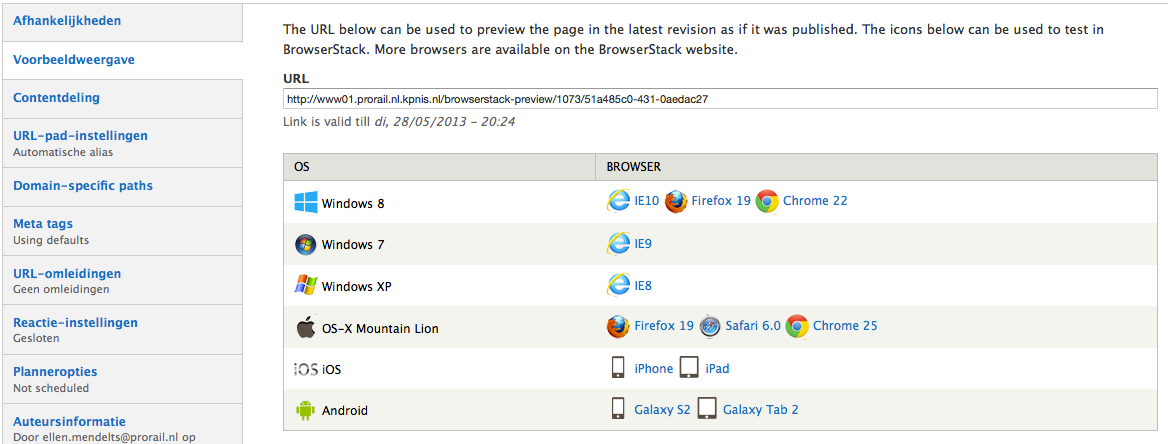
\includegraphics[width=\textwidth]{img/browserstack1.png}
\end{center}

Hier is een URL te zien die gebruikt kan worden om de pagina te bekijken. Hierop is altijd de laatste versie van de pagina te zien, zonder dat het nodig is om in te loggen. De link is beveiligd en is slechts 8 uur geldig, zie ook de datum onder de link. Met deze link kan de pagina zelf worden getest op een andere computer of mobiele telefoon, maar de pagina kan ook worden bekeken via \emph{Browserstack}. Dit is een dienst waarmee een breed scala aan browsers beschikbaar zijn om op te testen. Hierin zitten Windows, OS-X en mobiele platformen. Klik op \'{e}\'{e}n van de links in de tabel om de pagina direct in Browserstack te testen. Na het klikken op de link verschijnt het onderstaande scherm.

\begin{center}
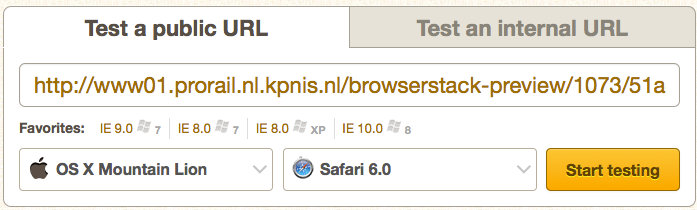
\includegraphics[width=\textwidth]{img/browserstack2.png}
\end{center}

Het kan nodig zijn om eerst in te loggen bij Browserstack voordat dit scherm te zien is. In dit scherm kunnen eventueel andere browsers worden gekozen. Hier zijn meer browsers beschikbaar dan in het vorige overzicht. De URL is vooraf ingevuld. Klik op "Start testing" om te pagina in de gekozen browser te bekijken.




\subsubsection{Scheduler}
\pvelist{ \pve{2.3.1}, \pve{2.3.9}, \pve{2.9.2}, \pve{2.9.3} }
Het is mogelijk om vooraf een publicatiedatum in te stellen voor nieuwe en bestaande inhoud. Klik hiervoor bij het toevoegen of bewerken van inhoud op de tab \emph{Planneropties}. Hier kunnen twee data worden opgegeven; een datum voor publicatie en een datum voor depublicatie. Biede velden zijn optioneel en werken in principe onafhankelijk van elkaar. Bij het klikken op \'{e}\'{e}n van deze velden verschijnt er een kalender waarop de datum kan worden gekozen.
\begin{center}
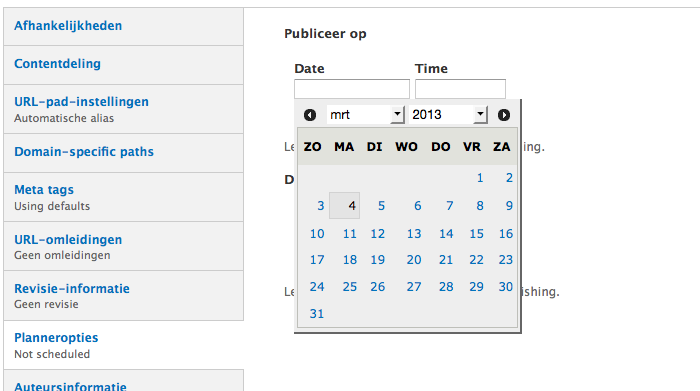
\includegraphics[width=\textwidth]{img/scheduler.png}
\end{center}
Niet gepubliceerde inhoud kan wel worden voorzien van tags, menu-items etc. Ook kunnen niet gepubliceerde items worden opgenomen in redactionele blokken\seeone{felix}. Zolang deze niet gepubliceerd is zal dit voor bezoekers niet zichtbaar zijn. Na publicatie (manueel of automatisch) wordt dit item zichtbaar.

Het (de)publiceren gebeurt in de cron (een achtergrond process dat om de 5 minuten draait) en kan daarom maximaal 5 minuten afwijken van de ingestelde tijd.




\subsection{Workflow en modereren/revisies}\label{workflow}
\pvelist{ \pve{2.2.5}, \pve{2.3.5}, \pve{2.3.6}, \pve{2.3.7}, \pve{2.3.10} }
In de website van ProRail wordt gebruik gemaakt van \emph{workflow}. Dat wil zeggen dat nieuwe inhoud en gewijzigde inhoud niet in alle gevallen direct op de site zal verschijnen, maar eerst goedgekeurd moet worden. Hierbij wordt onderscheid gemaakt tussen eindredacteuren en contentbeheerders. Contentbeheerders (ook wel "redacteur") kunnen enkel content binnen hun eigen subsite direct publiceren. Eindredacteuren hebben het recht om content binnen de gehele website te publiceren en aan te passen. Eindredacteuren kunnen content van contentbeheerders tevens publiceren op andere delen van de site.

De workflow is zowel van toepassing op nieuwe als bestaande inhoud. Bij reeds bestaande inhoud wordt een nieuwe \emph{revisie} aangemaakt. De nieuwe revisie kan bestaan naast de gepubliceerde pagina. Zo is het mogelijk dat een wijziging pas later - na goedkeuring - gepubliceerd wordt en dus zichtbaar voor bezoekers.

Bij het invoeren of bewerken van content is onderin het formulier een item "Publicatie-opties" te zien. Hierin staat een item "Moderatie status". Daarin zitten de volgende opties:
\begin{itemize}
\item Draft
\item Needs review
\item Published
\end{itemize}
Nieuwe inhoud of revisies worden als eerste aangemaakt als \emph{draft}. In deze staat is het een 'kladversie'. Bewerkingen hebben nog geen invloed op de website. Wanneer de content online mag dan kan de status op \emph{Needs review} worden gezet. In deze staat krijgen eindredacteuren dit item te zien in een lijst met goed te keuren inhoud. Tevens wordt een mail gestuurd naar alle eindredacteuren. Het item kan daarna op \emph{Published} worden gezet. De inhoud wordt dan zichtbaar op de website voor alle bezoekers. Afhankelijk van de rechten is het mogelijk om in dit proces stappen over te slaan.

\subsubsection{Revisies inzien en terugzetten}\label{modererentab}

De revisies van inhoud zijn later (ook na publicatie) terug te vinden onder het tabblad "Modereren". Op deze pagina is een lijst te zien waarin tevens de datum en workflow status te zien is. Met de link "weergeven" kan de revisie worden bekeken. Met de link "terugzetten" kan de revisie worden teruggezet. In het laatste geval publiceren we een oudere revisie, waarmee we alle latere wijzigingen ongedaan maken. Een revisie kan ook nieuwer zijn dan de versie die is gepubliceerd. In dit geval is er een "publiceren" link aanwezig. Hiermee kan deze versie worden goedgekeurd en gepubliceerd.

Onder de link "Vergelijk revisies" (2e niveau tabblad) zit een pagina waarmee makkeljik te verschillen tussen revisies zichtbaar gemaakt kunnen worden. Hierbij moeten twee revisies gekozen worden. Kies eerst de nieuwste revisie en daarna de oudere revisie (verder onderaan in de lijst). Klik daarna op de knop \emph{Vergelijken}. Hierna worden de tekstuele wijzigingen getoond. Dit heeft betrekking op de hoofdtekst van dit item.
\begin{center}
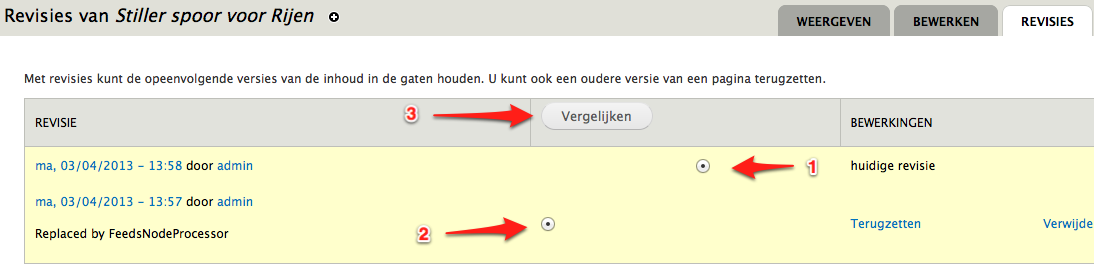
\includegraphics[width=\textwidth]{img/revisies3.png}
\end{center}

\subsubsection{Inhoud goedkeuren}

In het dashboard is voor eindredacteuren een lijst beschikbaar met inhoud dat goedgekeurd dient te worden. Dit is inhoud met de status \emph{Needs review}. Klik hiervoor linksboven op "Mijn Workbench" en dan op "Wacht op goedkeuring" (2e niveau tabblad). In deze lijst kan doorgeklikt worden naar de pagina's die goedgekeurd dienen te worden. Nadat de wijzigingen zijn bekeken kunnen deze worden goedgekeurd onder het tabblad "Modereren"\see{modererentab}.


\subsection{Contenttypes}

\subsubsection{Nieuws}
\pvelist{ \pve{4.13} }
%todo: screenshots

\subsubsection{Mini carousel}
\pvelist{ \pve{4.14} }

Om een slide toe te voegen aan een Onder de aandacht carrousel ga je eerst naar de taxonomie lijst van onder de aandacht en vul je een naam voor een carrousel in.

\begin{enumerate}
\item Klik op de link \emph{Inhoud toevoegen} of ga direct naar \drupalpath{node/add/slide}.
\item Vul de titel in van de slide
\item Klik op de \emph{Select media} button om een afbeelding te kiezen
\item Klik op \emph{Library} om een afbeelding te gebruiken die eerder is toegevoegd,  of voeg een nieuwe afbeelding toe via \emph{Upload a new file}
\item Vul een url in bij het \emph{Link} veld
\item Om de pagina op te slaan klik je onderaan de pagina op de knop \emph{Opslaan}
\item Om de slide aan een carousel toe te voegen wordt uitgelegd in \seeone{nodequeues}
\end{enumerate}
%todo: screenshots

\subsubsection{Infographics}
\pvelist{ \pve{4.16} }
\begin{enumerate}
\item Vul de titel in van de Infographic
\item Klik op de \emph{Select media} button om een afbeelding te kiezen
\item Klik op \emph{Library} om een afbeelding te gebruiken die eerder is toegevoegd,  of voeg een nieuwe afbeelding toe via \emph{Upload a new file}
\item Vul een url in bij het \emph{Link} veld
\end{enumerate}`
%todo: screenshots


\subsubsection{Storingen en werkzaamheden}
\pvelist{ \pve{4.17} }
Storingen en werkzaamheden zijn te bekijken via de pagina \drupalpath{reizigers/storingen}. Als de bezoeker op een storing klikt verschijnt er meer informatie, zoals de reden van de storing, extra reistijd en andere relevante informatie die uit de NS API komt.

Om storingen te tonen op andere pagina's kan de redacteur blokken toevoegen via Felix, de blokken die over storingen en werkzaamheden gaan zijn:

\begin{enumerate}
\item Laatste 3 storingen
\item Alle storingen
\item Alle werkzaamheden
\end{enumerate}`

De storingen en werkzaamheden kunnen ook bekeken worden via RSS: \drupalpath{storingen/rss}.

%todo: screenshots

\subsubsection{Navigatie blokken}
\pvelist{ \pve{4.19} }
%todo: screenshots

\subsubsection{Downloads}
\pvelist{ \pve{4.20} }
\begin{enumerate}
\item Vul de titel in van het Redactionele blok
\item Voeg de content toe in het \emph{Body} veld
\item Vul een url in bij het \emph{Link} veld
\item Klik op de \emph{Select media} button om een afbeelding te kiezen
\item Klik op \emph{Library} om een download te gebruiken die eerder is toegevoegd,  of voeg een nieuwe download toe via \emph{Upload a new file}
\item De downloads worden weergeven als het blok toegevoegd is via Felix
\end{enumerate}
%todo: screenshots

\subsubsection{Standaard pagina}\label{pagenode}
\pvelist{ \pve{4.21} }
%todo: screenshots

\subsubsection{Fotoalbum}
\pvelist{ \pve{4.22} }
Bij het toevoegen van afbeeldingen bij bijvoorbeeld een nieuwsartikel, heeft de redacteur de mogelijkheid om een fotoalbum te maken. Als de redacteur meer dan 1 afbeelding aan het nieuwsbericht toevoegt verschijnt er automatisch bij dat nieuwsbericht een fotoalbum. De foto's dienen breder te zijn dan 588, anders komt het niet in het fotoalbum terecht.

Afbeeldingen via Flickr kunnen toegevoegd worden via de embed code van Flickr.

Om Flickr sets toe te voegen op de website kan door middel van Felix. Kies hiervoor voor Flickr set en vul het gebruikersnummer en de setnummer in.

\subsubsection{Stel een vraag}
\pvelist{ \pve{4.23} }
%todo: screenshots

\subsubsection{Contactformulier}
\pvelist{ \pve{4.24} }

Het contacformulier staat op \drupalpath{contact}. Deze pagina is standaard leeg. Alle content wordt geplaatst via Felix\seeone{felix}.

%todo: screenshots

\subsubsection{Poll}
\pvelist{ \pve{4.26} }
Ga naar Inhoud $\Rightarrow$ Inhoud toevoegen $\Rightarrow$ Enqu\^{e}te, of direct naar drupalpath{node/add/advpoll}. De volgende velden zijn beschikbaar.
\begin{enumerate}
\item Vraag, de vraag en tevens titel van de poll.
\item Beschrijving, een eventuele omschrijving bij de vraag.
\item Poll choice, de antwoorden waarop een gebruiker kan stemmen. Via de knop Item toevoegen kan je extra vragen toevoegen.
\item Poll availability, kies hier tussen welke data de poll open moet zijn. Buiten deze periode is de poll nog wel zichtbaar maar kan er niet gestemd worden.
\item Close poll, kies hier of de poll open en gesloten moet zijn. Je kan hiermee de poll sluiten ook wanneer hij nog binnen het termijn valt.
\end{enumerate}

Via Felix kan een poll worden geplaatst op de website.


\subsubsection{Project}\label{projectnode}


\subsubsection{Carousel}
\pvelist{ \pve{4.14} }
\begin{enumerate}
\item Klik op de link \emph{Inhoud toevoegen} of ga direct naar \
\item Vul de titel in van de slide
\item Klik op de \emph{Select media} button om een afbeelding te kiezen
\item Klik op \emph{Library} om een afbeelding te gebruiken die eerder is toegevoegd,  of voeg een nieuwe afbeelding toe via \emph{Upload a new file}
\item Vul een url in bij het \emph{Link} veld
\item Om de pagina op te slaan klik je onderaan de pagina op de knop \emph{Opslaan}
\item Om de slide aan een carousel toe te voegen wordt uitgelegd in \seeone{nodequeues}
\end{enumerate}
%todo: screenshots

\subsubsection{Systeempagina}
\pvelist{ \pve{2.6.4} }
Systeempagina's zijn gelijk aan een standaard pagina\seeone{pagenode} met het verschil dat een systeempagina niet wordt opgenomen in de zoekresultaten. Dit wordt bijvoorbeeld gebruikt voor de foutpagina's, maar kan door redacteuren ook voor andere pagina's worden gebruikt waarvan niet wenselijk is dat deze in de zoekresultaten voorkomen.

\subsubsection{Cookiebalk}
Via \drupalpath{admin/config/user-interface/cookie-consent} kunnen de instellingen voor de cookiebalk worden aangepast. Hier kan bijvoorbeeld de link voor meer informatie worden aangepast. Ook kunnen domeinen uitgesloten worden van deze functionaliteit (dient alleen gebruikt te worden voor domeinen die niet publiekelijk bereikbaar zijn).

\subsubsection{Twitterberichten}
\begin{enumerate}
\item Ga naar de pagina waar de Twitterberichten getoond moeten worden
\item Kies de Felix regio en klik via het tandwieltje op \emph{Add block}
\item Klik op \emph{Twitter}
\item Geef een titel op en een gebruikersnaam, in dit geval wordt dat \emph{prorail}
\item Klik op \emph{Opslaan}
\end{enumerate}
%todo: screenshots

\subsubsection{Handige links blok}
\begin{enumerate}
\item Vul de titel in van het Redactionele blok
\item Voeg de content toe in het \emph{Body} veld, hier worden de links ingevoerd. \\
Links naar bestanden moeten beginnen met een slash (bijvoorbeeld: \\ "/sites/default/files/document.pdf").
\item Klik op \emph{Opslaan}
\item Plaats met Felix dit Redactionele blok op een pagina
\end{enumerate}
%todo: screenshots

\subsubsection{Vrij blok}
\begin{enumerate}
\item Vul de titel in van het Redactionele blok
\item Voeg de content toe in het \emph{Body} veld
\item Vul een url in bij het \emph{Link} veld
\item Plaats met Felix dit Redactionele blok op een pagina
\end{enumerate}
%todo: screenshots

\subsubsection{Hoofdnavigatie}
%todo: screenshots

\subsubsection{Projectmenu}
%todo: screenshots

\subsubsection{Toevoegen veelgestelde vraag}

\begin{enumerate}
\item Ga naar Inhoud $\Rightarrow$ Inhoud toevoegen $\Rightarrow$ Veelgestelde vraag of direct naar \drupalpath{/node/add/faq}.
\item De volgende velden kunnen ingevoerd worden; vraag en body.
\end{enumerate}

\subsubsection{Koppelen van een veelgestelde vraag aan content}

\emph{Dit geldt voor zowel projecten als onderwerpen}

\begin{enumerate}
\item Bewerk of maak een nieuw project/onderwerp aan.
\item Bij het onderdeel Koppel veelgestelde vragen kan je middels een autocomplete veld vragen zoeken en koppelen aan het item.
\item Sla daarna het project/onderwerp op.
\end{enumerate}

\subsubsection{Project}

Een voorbeeld van een project waar vragen aan gekoppeld zijn is http://prorail.staging.dop.nu/hanzelijn. Hierbij is het laatste blok onder de content de veelgestelde vragen-accordion.

De overzichtspagina van alle vragen bij een project is te vinden op http://prorail.staging.dop.nu/node/29/vragen. Voor de URL moet nog een nette oplossingen gevonden worden.

\subsubsection{Onderwerp}

Een voorbeeld van een onderwerp waar vragen aan gekoppeld zijn is te vinden op http://prorail.staging.dop.nu/omwonenden/vervoer. Hierbij staan de vragen aan de rechterkant van de content.

\subsubsection{Prestatiecijfers / infographics}
\pvelist{ \pve{4.16} }
Prestatiecijfers en Infographics kunnen worden toegevoegd via Inhoud $\Rightarrow$ Inhoud toevoegen $\Rightarrow$ Infographic of direct naar \drupalpath{/node/add/infographic}. Bij afbeelding kan een Infographic worden geupload. Via Felix kan dan een Infographic worden getoond op de website.

\subsubsection{Filterblok}
Het filterblok is beschikbaar als Felixblok. Het blok heet View: Categorieen: Block.
\subsubsection{Aanmaken Live blog nieuws}
Ga naar \drupalpath{/node/add/blognieuws} en voer een titel en body tekst op

\subsubsection{Aanmaken live blog update}

Ga naar \drupalpath{/node/add/blogpost}
Vul de volgende velden in titel, body, foto en video
Vul bij Liveblog nieuws endpoints de titel van de aangemaakte live blog nieuws in om hem te koppelen.

\subsubsection{Live blog blok tonen}

Ga naar de voorpagina en selecteer in felix bij eerste helft het blok View: Liveblog: Belangrijk nieuwsblok

Standaard worden alle Felixblokken helemaal onderaan gezet en kunnen met move up bovenaan gezet worden.
\subsection{Content bewerken}

\pvelist{ \pve{2.2.1}, \pve{2.2.4} }

\begin{enumerate}
\item Ga naar \emph{Mijn Workbench} $\Rightarrow$ \emph{Inhoud zoeken} of ga direct naar \drupalpath{admin/workbench/all-content}, je zult nu de pagina te zien krijgen waar alle inhoud te vinden is.
\item Om de gewenste inhoud sneller te vinden kun je de filterfunctie gebruiken, bovenaan de pagina. Klik bijvoorbeeld bij het label "type" in het lijstje op "Standaard content item" en vervolgens klik je op "Toepassen". Alleen artikelen van het type "Standaard content item" zullen nu getoond worden.
\item Zoek naar de titel van het artikel dat je wilt gaan bewerken en klik vervolgens op "bewerken" in de meest rechtse kolom genaamd "handelingen".
\item Je bent nu gereed om de content te gaan bewerken. Om de bewerkingen op te slaan klik je onderaan de pagina op de knop "Opslaan".
\end{enumerate}

De bestaande pagina blijft tijdens de bewerkmodus beschikbaar voor bezoekers.

Het is niet mogelijk om met meerdere redacteuren aan dezelfde pagina te werken. Het bewerkscherm is toegankelijk, maar bij het opslaan zal de volgende melding verschijnen: \emph{"De inhoud op deze pagina is gewijzigd door een andere gebruiker, of u heeft al wijzigingen ingediend via dit formulier. De wijzigingen kunnen daardoor niet worden opgeslagen."}.

\subsubsection{Hoe plaats je een afbeelding naast een stuk tekst}
Dit kun je doen door de afbeelding toe te voegen in de lopende tekst. Rechtermuisknop op de afbeelding en kies dan voor eigenschappen.Onderaan kun je kiezen voor de uitlijning.
%todo: https://dutchopen.unfuddle.com/a#/projects/106/tickets/by_number/253 screenshots
\subsection{Standaardvelden}
Alle content typen bevatten verschillende standaardvelden. De onderstaande lijst beschrijft elk veld apart.

\subsubsection{Titel}
De titel van de pagina, dit veld is altijd verplicht.

\subsubsection{Intro tekst}
De intro tekst van de pagina, dit veld is bij de meeste content typen niet verplicht. Deze tekst zal als introductie teaser worden getoond.

\subsubsection{Body tekst}
Dit veld is het meest belangrijk, in dit veld dient de hoofdtekst ingevuld te worden. Gebruik de editor om de tekst te stijlen met bijvoorbeeld vet gedrukte of cursieve teksten.

\subsubsection{Afbeeldingen}
Klik op �Selecteer media� bij het veld �Afbeeldingen�, selecteer een afbeelding en klik op �toevoegen�. Klik vervolgens op �Item toevoegen�. Herhaal deze stappen indien je meerdere afbeeldingen wil toevoegen.

\subsubsection{Media}\label{media}
\pvelist{ \pve{2.16} }
Klik op �Select media� bij het veld �Media�, selecteer een bestand en klik op �Indienen�. Indien je meerdere mediabestanden wilt toevoegen klik je op �Item toevoegen� en klik vervolgens op �Select media�.

Het is ook mogelijk om een video van het web toe te voegen. Klik op �Select media� bij het veld �Media�. Klik vervolgens op de tab �Web�. Bij het veld �URL or embed code� vul je de URL of embed code in. Dit is een voorbeeld URL om een youtube video toe te voegen:  \texttt{http://www.youtube.com/embed/Abiil-lD3HY} . Om het bestand toe te voegen klik je op �Indienen�.

Ook kan er een bestand uit de bibliotheek toegevoegd worden. Klik op �Select media� bij het veld �Media�. Klik vervolgens op de tab �Bibliotheek� en selecteer het gewenste bestand. Om het bestand toe te voegen klik je op �Indienen�. Toegestane bestandstypen zijn: �avi� (= video) en �mp3� (= audio).

\subsubsection{Attachments}
Klik op �Selecteer media� bij het veld �Attachments�, selecteer een bestand en klik op �toevoegen�. Klik vervolgens op �Item toevoegen�. Herhaal deze stappen indien je meerdere bestanden wil toevoegen.

\subsubsection{Tekstopmaak}
\pvelist { \pve{2.18} }
Onder het veld �Body� kan telkens gekozen worden tussen drie verschillende opties: �Filtered HTML�, �Full HTML� en �Plain text�.
\begin{itemize}
\item Filtered HTML: voorgedefinieerde HTML tags zullen worden toegestaan, alle overige HTML tags zullen uit de tekst gefilterd worden.
\item Full HTML: alle HTML tags zijn toegestaan.
\item Plain text:  alleen gewone tekst is toegestaan, alle HTML of andere code zal gefilterd worden zodra de pagina wordt opgeslagen.
\end{itemize}
Binnen \emph{Filtered HTML} is het mogelijk om \emph{iframes} toe te voegen. Dit zijn embedded webpagina's van andere websites. Deze kunnen worden gebruikt om 3th party modules zoals bijv. een enqu\^{e}te in te sluiten.

\subsubsection{Locatie}
Het locatieveld is beschikbaar in de volgende content types: Webformulier, Agenda, Bekendmaking, Bestemmingsplan, Pagina, Nieuws, Product. De veld bestaat uit twee onderdelen. Het eerste is het invullen van adres gegevens. Deze bestaat uit een locatienaam, de straat, de postcode, de woonplaats en het land. De waardes die hier ingevuld worden zullen gebruikt worden om de Google Maps link te genereren.

\begin{center}
	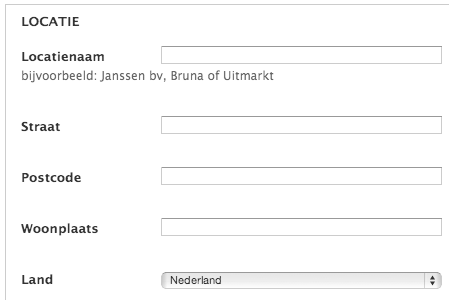
\includegraphics[width=\textwidth]{img/locatie1.png}
\end{center}

Het tweede deel van dit veld is een kaart met daaronder twee velden, Breedtegraad en Lengtegraad. Dit deel wordt gebruikt om het kaartje te tonen in de rechterkolom van een detailpagina. Er zijn twee manieren waarop een locatie aangegeven kan worden. Dat is door op de kaart te klikken en de pointer er neer te zetten. Of wanneer je de exacte breedte- en lengtegraad weet, deze in te vullen.

\begin{center}
	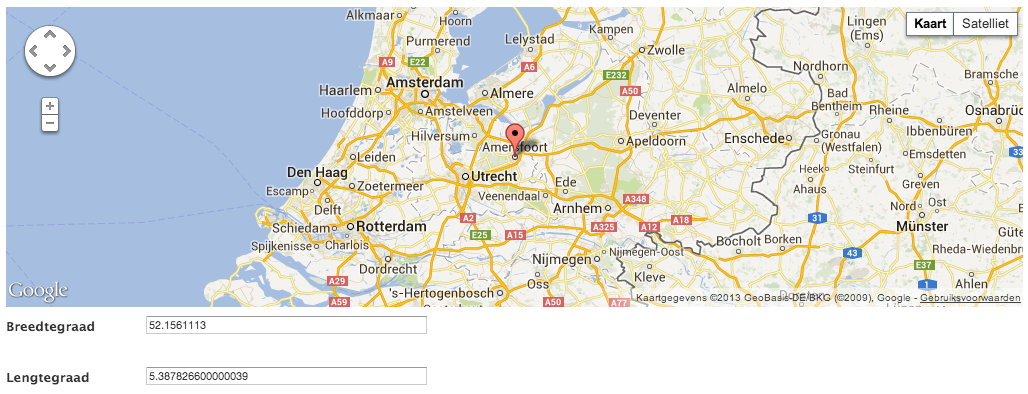
\includegraphics[width=\textwidth]{img/locatie2.png}
\end{center}

\subsubsection{URL alias}\label{alias}
\pvelist{ \pve{2.6}, \pve{2.6.1}, \pve{2.6.2} }
Nieuwe inhoud wordt automatisch op een vriendelijke URL geplaatst (bijv. \\ \texttt{\customerdomain /nieuws/2013/onderwerp}). Dit pad zal normaliter niet aangepast hoeven te worden. De \emph{URL alias} geeft het \emph{gebruikelijke} pad van de pagina weer. 

Het uitgangspunt is dat het automatische pad gehanteerd wordt, maar indien dit onwenselijke resultaten oplevert dan is het voor redacteuren wel mogelijk om dit pad aan te passen. Klik hiervoor bij het toevoegen of bewerken van inhoud op \emph{URL-pad-instellingen} (onderaan de pagina). Daar staat een checkbox die aangeeft dat er een automatische URL gebruikt wordt. Na het uitvinken hiervan kan eronder in een tekstveld een eigen pad worden aangegeven. 

Het is mogelijk om speciale tekens te gebruiken in de URL alias. Echter raden we het gebruik daarvan sterk af. In veel browsers worden deze getoond met een andere codering (een apostrof wordt bijvoorbeeld "\%E2\%80\%89"). Aanbevolen wordt om de tekens te beperken tot alfanumeriek (a t/m z en 0 t/m 9) en afbreekstreepjes. Het gebruik van hoofdletters is ook niet gebruikelijk in URL's.

\subsubsection{Publiceren onder embargo (Planneropties)}
Publiceren onder embargo is te vinden tussen de horizontale tabs bij het bewerken van een item. Het gaat om de tab \emph{Planneropties}.

Deze tab bevat een aantal datum/tijd velden.
\begin{itemize}
\item Publiceer revisie op \emph{(alleen bij bewerken)}
\item Publiceer op
\item Depubliceer op
\end{itemize}

Geen van de velden is verplicht en kunnen afzonderlijk van elkaar ingevuld worden. Wanneer alleen de \emph{Publiceer op} ingevuld wordt zal het item pas gepubliceerd worden na deze datum. Wanneer alleen \emph{Depubliceer op} ingevuld wordt zal het item na deze datum niet meer verschijnen. Worden beide velden ingevuld zal het item alleen tussen deze twee datums getoond worden.

De velden \emph{Publiceer op} en \emph{Depubliceer op} gaan over het (de)publiceren van de volledige node. Het is ook mogelijk om wijzigingen aan te brengen op een reeds gepubliceerd item, waarbij die wijzigingen op een bepaalde datum worden gepubliceerd. Daarvoor moet een datum worden ingevuld bij \emph{Publiceer revisie op}. De moderatie status onder \emph{Publicatie-opties} laat men in dat geval op \emph{Concept} staan, aangezien dat veld over de \emph{actuele} status gaat.

\subsection{Tags}
\pvelist{ \pve{2.14.4} }
Het is mogelijk om trefwoorden (tags) toe te voegen aan inhoud\seeone{trefwoorden}. In het beheergedeelte is een lijst beschikbaar van alle trefwoorden. Ga hiervoor naar \emph{Structuur} $\rightarrow$ \emph{Taxonomie} en klik rechts van \emph{Tags} op \emph{termen weergeven}. De pagina is ook direct beschikbaar op \drupalpath{admin/structure/taxonomy/tags}.

Klik rechts van een tag op \emph{bewerken} om een tag aan te passen of om deze te verwijderen. Hier kunnen bijvoorbeeld taalfouten uit de naam worden gehaald. Verander daarvoor de naam in het naam-veld en klik onderaan op \emph{Opslaan}. Onwenselijke tags kunnen weggehaald worden door op de knop \emph{Verwijderen} te klikken. Het is dan niet nodig om de inhoud te bewerken die gebruik maakt van deze tags.

\subsection{Nieuwscategorie}
Het is mogelijk om nieuwscategorien aan te maken via \drupalpath{admin/structure/taxonomy/categorieen}. Op  https://\drupalpath{nieuws} kan de bezoeker filteren.
\subsection{Downloads}
\label{sec:Downloads}
De inhoud van dit blok wordt gevuld vanuit een nodequeue. De redactie kan de inhoud van dit blok zelf samenstellen. Bestanden kunnen gekoppeld worden aan daarvoor bestemde inhoudstype. Deze nodes kunnen dan gekozen worden in een nodequeue. Het blok zal daarna een lijst tonen met de bestandsnaam, de extensie en de grootte van het gekoppelde bestand. Na het klikken op de bestandsnaam zal er een download dialoogvenster van de browser geopend worden.
\subsection{Nodequeues}\label{nodequeues}
Nodequeues zijn kort omschreven: \emph{wachtrijen voor content items (nodes)}. In een nodequeue kun je precies bepalen welke content er weergegeven wordt, het aantal en de volgorde van de toegevoegde content items.

\subsubsection{Nodequeues aanmaken}
Klik op de link �Structuur� en klik vervolgens op �Nodequeues� of ga direct naar \drupalpath{admin/structure/nodequeue}. Bovenaan de pagina verschijnen twee links: �exams queue toevoegen� en �simple queue toevoegen�.
Klik op �simple queue toevoegen� om een nodequeue aan te maken.

Je zult nu op de pagina terecht komen waar je een nieuwe queue kunt toevoegen.
\begin{enumerate}
\item Vul een titel in om de wachtrij een naam te geven
\item Limiteer hoeveel content items er kunnen worden getoond in de wachtrij, vul �0� (nul) in voor een onbeperkt aantal.
Kruis het vakje aan bij �Reverse in admin view� indien je content items vooraan de wachtrij wil toevoegen i.p.v. achteraan de wachtrij. 
\item Sla de stappen bij de velden �Link �add to queue� en �remove from queue� text� over.
\item Kruis aan bij �Rollen� welke gebruikers content items aan de nodequeue kunnen toevoegen.
\item Kruis aan bij �Typen� welke content items behorende bij de content typen toegevoegd kunnen worden aan de nodequeue.
\end{enumerate}

\subsubsection{Content toevoegen aan nodequeues}

Klik op de link �Structuur� en klik vervolgens op �Nodequeues� of ga direct naar \drupalpath{admin/structure/nodequeue}. Indien je al nodequeues hebt aangemaakt zal op deze pagina een lijst geladen worden met alle aangemaakte nodequeues. Klik op �Weergeven� in de meest rechter kolom om de wachtrij te tonen met alle toegevoegde content items. 

In het veld welke gevuld is met de tekst �Enter the title of a node to add it to the nodequeue�, vul je (deels) de titel in van het content item dat je aan de wachtrij wilt toevoegen. De titel hoef je slechts deels in te vullen omdat de website de titel automatisch zal aanvullen (indien de titel bestaat). Klik op de gevonden titel en klik vervolgens op �Inhoud toevoegen�.

Herhaal deze stappen om meerdere content items aan de nodequeue toe te voegen. Vervolgens kun je alle content items sorteren: handmatig, met de knop �omkeren� of �shuffle�.
\begin{itemize}
\item Handmatige sortering: houdt de muis ingedrukt op het kruisje in de meest linker kolom, sleep vervolgens het content item naar de gewenste positie. Wanneer je klaar bent met handmatig sorteren klik je op �Opslaan�.
\item Knop �omkeren�: draait de wachtrij volledig om
\item Knop �shuffle�: sorteer de wachtrij op willekeurige volgorde.
\end{itemize}



\subsection{Contentdeling}\label{contentdeling}
\pvelist{ \pve{2.13}, \pve{2.13.1}, \pve{2.13.2}, \pve{2.13.3}, \pve{2.13.4} }
Het is mogelijk om inhoud op meerdere subsites te gebruiken. Een nieuwsartikel kan bijvoorbeeld zichtbaar zijn op de subsites van zowel reizigers als omwonenden.

Bij het toevoegen of bewerken van een node staat er onderin het formulier een item \emph{Contentdeling}. Na het klikken op de link \emph{Contentdeling} wordt een lijst getoond met alle subsites. Vink de subsites aan waarop de inhoud beschikbaar moet zijn. Het is verplicht om minimaal \'{e}\'{e}n subsite aan te vinken. Onder de lijst van domeinen kan een brondomein worden gekozen. Dit domein (subsite) wordt gebruikt als \emph{canonical url}. Dit is de URL die door zoekmachines zal worden gebruikt om de pagina te indexeren. Tevens wordt deze subsite gebruikt wanneer naar dit item wordt gelinkt vanuit een andere subsite waar dit item niet is gepubliceerd. Bij het aanmaken van nieuwe inhoud is standaard het huidige domein als brondomein geselecteerd.


\subsection{Flexible blokken}\label{felix}
Het is voor redacteuren mogelijk om blokken de plaatsen op pagina's. Hiermee krijgt de redacteur enige vrijheid over de indeling van de pagina. Hier zijn wel beperkingen van toepassing volgens het grafisch ontwerp.

Door met de muis over de grijze balk te gaan verschijnt er een tandwieltje, als je daarop klikt dan verschijnt er een optie \emph{Blok toevoegen}. Hier kan een keuze gemaakt worden om een enkel item weer te geven op de website, dit zijn \emph{Nodetypes}, of een aantal items, zoals bijvoorbeeld \emph{Het laatste nieuws}.

\begin{center}
	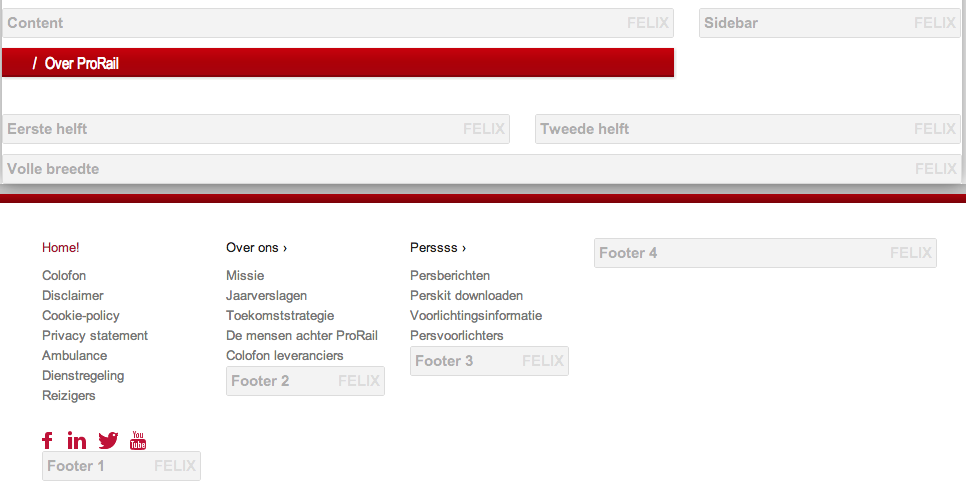
\includegraphics[width=\textwidth]{img/felix.png}
\end{center}
\section{Menu}\label{menu}
Via een aparte sectie in de beheeromgeving kunnen de beschikbare menu's worden aangepast. Het menu systeem staat in Drupal los van de inhoud (nodes). Om een pagina in het menu toe te voegen zal eerst de pagina toegevoegd moeten worden en kan daarna het menu-item worden aangemaakt.

\subsection{Menu-items toevoegen}\label{menuitemstoevoegen}
menu items toevoegen tekst

\subsection{Menu-items bewerken}\label{menuitemsbewerken}
menu items bewerken tekst
\subsection{Afbeeldingen}
\pvelist{ \pve{2.15} }

Afbeeldingen worden automatisch geschaald in verhouding naar aanleiding van het design. De originele afbeelding wordt bewaard op de server: Een voorbeeld:

Originele afbeelding: http://accept.prorail.nl.kpnis.nl/sites/default/files/nachtelijk\_onderhoud\_aan\_het\_spoor\_300dpi\_451x300mm\_c.jpg
Geschaald: http://accept.prorail.nl.kpnis.nl/sites/default/files/styles/960x437/public/nachtelijk\_onderhoud\_aan\_het\_spoor\_300dpi\_451x300mm\_c.jpg

Als er een afbeelding wordt toegevoegd in de WYSIWYG editor heeft de gebruiker de keuze om drie formaten te kiezen:

\begin{enumerate}
\item Standaard, De afbeelding wordt net zo groot als het content vlak
\item Teaser, De afbeelding wordt net zo groot als een afbeelding in het overzicht
\item Origineel, De afbeelding wordt net zo groot als het is geupload
\end{enumerate}

\begin{figure}[p]
\centering
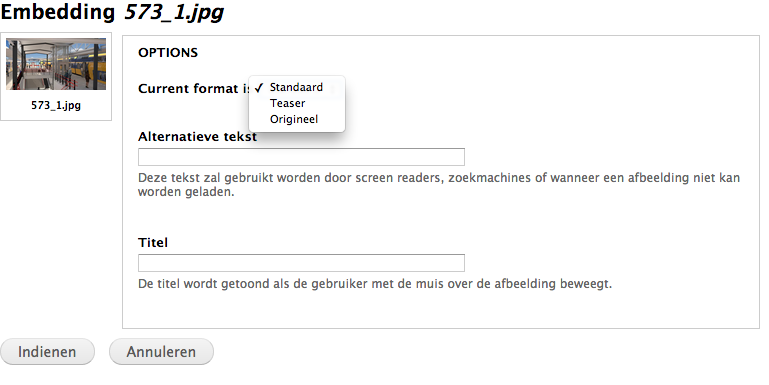
\includegraphics[width=\textwidth]{img/wysiwyg_image.png}
\caption{De drie aanwezige formaten om een afbeelding toe te voegen aan de tekst}
\label{fig:felix_image}
\end{figure}

Bij het toevoegen van afbeeldingen bij bijvoorbeeld een nieuwsartikel, heeft de redacteur de mogelijkheid om een fotoalbum te maken. Als de redacteur meer dan 1 afbeelding aan het nieuwsbericht toevoegt verschijnt er automatisch bij dat nieuwsbericht een fotoalbum.

Afbeeldingen via Flickr kunnen toegevoegd worden via de embed code van Flickr.

Om Flickr sets toe te voegen op de website kan door middel van Felix. Kies hiervoor voor Flickr set en vul het gebruikersnummer en de setnummer in.
\subsection{Wysiwyg en media}\label{wysiwyg}

Voor media en wysiwyg worden de \usemodule{wysiwyg} en \usemodule{media} / \usemodule{file\_entity} modules ingezet. Als editor zelf wordt gekozen voor \texttt{CKEditor} aangezien dit de meestgebruikte editor is binnen Drupal en standaard is in Drupal 8.

\subsubsection{Buttons}

De buttons staan gespecificeerd in het FO document.
Een aantal buttons zit niet standaard in de \usemodule{wysiwyg} module. Hiervoor wordt de reeds ontwikkelde \texttt{ckeditor\_customtags} module gebruikt waarmee buttons kunnen worden toegevoegd.

\subsubsection{Links in bodytekst}

Voor het gemakkelijk kunnen toevoegen van links in bodyteksten wordt gebruik gemaakt van de \usemodule{linkit} module i.c.m. \usemodule{pathologic}.

\subsubsection{Invoerformaten}\label{invoerformaten}

Er worden drie invoerformaten ter beschikking gesteld voor gebruikers en redacteuren.

\begin{itemize}
\item \textbf{Full HTML} \\
Volledige HTML zonder filtering. Alleen beschikbaar voor eindredacteuren. Het wordt aanbevolen om hier spaarzaam gebruik van te maken vanwege de mogelijkheid om nieuwe XSS issues (security issues) te introduceren.
\item \textbf{Filtered HTML} \\
Standaard filtering op ongewenste HTML en herschrijven van links door \texttt{pathologic}.
\item \textbf{Plain text} \\
Wordt gebruikt voor reviews (geplaatst door bezoekers). Hierbij wordt geen opmaak / HTML toegestaan.
\end{itemize}

\subsubsection{Media}\label{media}

Images en video's moeten toegevoegd en hergebruikt kunnen worden in wysiwyg en bestandsvelden.
Uitgangspunt is versie 2 van de \texttt{media} module.




\subsection{Zoeken}\label{zoeken}

Voor \drupalpath wordt de \emph{Solr module} gebruikt, deze module vervangt de standaard \emph{Drupal Search module}. 
De \emph{Solr module} biedt naast de standaard zoek functionaliteit ook meer geavanceerde functionaliteiten zoals zoeken in bijlagen, markeren van zoekwoorden en de mogelijkheid tot het aanpassen van de \emph{Bias settings}. 

\subsubsection{Bias settings}

\emph{Bias settings} maken het mogelijk inhoud voorrang te geven in de zoekresultaten. Je kunt bijvoorbeeld het inhoudstype \emph{Nieuws} meer punten geven dan het inhoudstype \emph{Bekendmaking}. Hoe hoger het aantal toegekende punten hoe meer voorrang het krijgt. 

Ga naar \drupalpath{admin/config/search/apachesolr} en klik vervolgens op \emph{Bias} bij de betreffende website om de \emph{Bias settings} aan te passen. Let op: het is niet aangeraden om zonder voldoende kennis deze settings aan te passen.

\begin{center}
	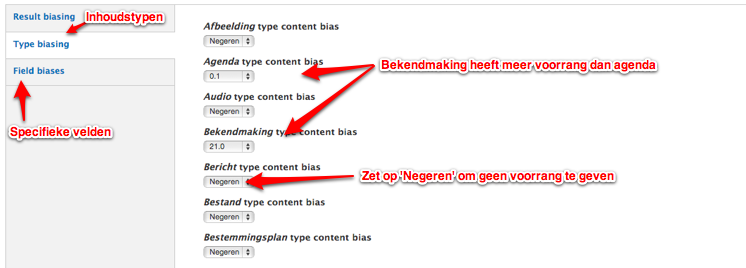
\includegraphics[width=\textwidth]{img/bias.png}
\end{center}

Klik na het bewerken op de knop \emph{Instellingen opslaan} om de \emph{Bias settings} op te slaan. 

\subsubsection{Content uitsluiten van zoekmachine}

Het is mogelijk om specifieke nodes uit te sluiten van indexatie in de interne zoekmachine. Klik onderaan het bewerkformulier op het tabblad \emph{Uitsluiten uit zoekresultaten} en vink de checkbox aan, zie onderataand afbeelding.

\begin{center}
	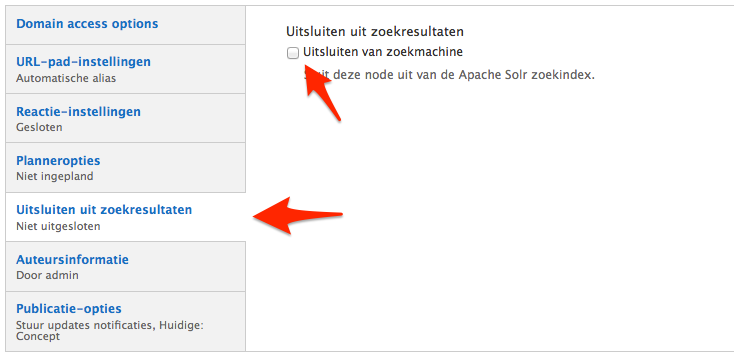
\includegraphics[width=\textwidth]{img/solr-exclude.png}
\end{center}

\subsubsection{Synoniemen beheren}

Solr biedt ondersteuning voor synoniemen. Hiermee kan worden ingesteld dat een zoekopdracht naar "i-pad" ook inhoud met de tekst "ipad" wordt opgenomen in de resultaten.

De synoniemen zijn te beheren via Drupal. Ga hiervoor naar \\ \drupalpath{admin/config/search/apachesolr/synonyms}. Op deze pagina is een lijst te vinden met de huidige synoniemen. Deze kunnen hier worden aangepast of uit de lijst worden gehaald. Onder de lijst is een formulier zichtbaar waarmee nieuwe synoniemen toegevoegd kunnen worden. Het trefwoord is het originele woord (bijv. "ipad") en de synoniemen worden ingevoerd als een komma gescheiden lijst (bijv. "i-pad, i pad").

Nieuwe synoniemen treden niet direct in werking. De lijst wordt iedere nacht doorgezet naar de Solr server. In dit proces wordt tevens de ingestelde lijst samengevoegd met de basislijst (generieke lijst voor alle gemeentes).

\section{Instellingen}


\subsection{Vertalen}
\pvelist{ \pve{2.10} }
Alle teksten die in de website worden gebruikt en geen deel uitmaken van de paginainhoud kunnen worden vertaald via de Drupal vertaalinterface. Deze interface is beschikbaar op \emph{Instellingen} $\rightarrow$ \emph{Interface vertalen} of direct op \drupalpath{admin/config/regional/translate}. Klik op het tabblad \emph{Vertalen}.

Via het formulier bovenin kan worden gezocht naar teksten op de website. Vul hiervoor (een deel van) de tekst in die vertaald moet worden. Deze zoekfunctionaliteit is hoofdlettergevoelig.

Klik in de lijst van teksten op \emph{bewerken} om een vertaling in te voeren.

\subsection{Calamiteiten pagina}
\pvelist{ \pve{4.1.1.2, 4.4} }
Om de site in calamiteiten mode te zetten ga je als volgt te werk:

\begin{enumerate}
\item Ga naar \drupalpath{node/237/edit} om de calamiteiten pagina te bewerken indien nodig
\item Controleer of de calamiteitenpagina is gepubliceerd
\item Ga naar \emph{Structuur} $\rightarrow$ \emph{Dominion} of direct naar \drupalpath{admin/structure/dominion/list/1/edit}
\item Vul bij \emph{voorpagina} de tekst \emph{calamiteiten} in
\item Klik op Oplaan
\end{enumerate}

Op de calamiteitenpagina heeft de redacteur alle vrijheid om blokken te plaatsen, net zoals alle andere pagina's.

\begin{figure}[p]
\centering
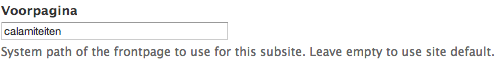
\includegraphics[width=\textwidth]{img/calamiteiten.png}
\caption{Calamiteiten pagina activeren}
\label{fig:calamiteiten_image}
\end{figure}

\section{Projecten}

Binnen \customerdomain is er de mogelijkheid om projecten aan te maken. Projecten zijn technisch gezien \emph{subsites}. Deze kunnen worden beheerd op \emph{Structuur} $\rightarrow$ \emph{Dominion} of direct op \drupalpath{admin/structure/dominion}.

\subsection{Project toevoegen}\label{projecttoevoegen}

Klik in het subsites overzicht op \emph{Add project subsite} of ga direct naar \\ \drupalpath{admin/structure/dominion/add/project}. In het formulier moeten de volgende gegevens worden ingevuld:
\begin{itemize}
\item Naam: naam van de subsite (bijv. "Hanzelijn")
\item Domain type: klik op \emph{Use a directory}
\item Directory: vul het pad van de subsite in (bijv. "projecten/hanzelijn")
\end{itemize}
De laatste optie is alleen zichtbaar wanneer \emph{directory} als \emph{domain type} is opgegeven. Binnen de Prorail site is het de conventie om het pad te beginnen met "projecten/". Het wordt tevens aanbevolen om enkel kleine letters te gebruiken aangezien het pad hoofdlettergevoelig is en hoofdletters in URL's niet gangbaar zijn.

Op het ingevoerde pad zal de subsite zichtbaar worden. Hierop is ook de projectnode te zien aangezien dat de voorpagina is van de subsite. De node zelf heeft daarom geen alias.

\subsection{Project wijzigen}

Waar een wijziging voor een project doorgevoerd moet worden is afhankelijk van de aard van de wijziging. Kortweg:
\begin{itemize}
\item Naam van subsite
\begin{itemize}
\item In de titelbalk $\rightarrow$ dominion
\item Titel op de voorpagina en naam op kaart $\rightarrow$ bewerk project node
\item Naam op menu-item naar voorpagina $\rightarrow$ bewerk menu-item
\end{itemize}
\item Pad van subsite $\rightarrow$ dominion
\item Tekst van de voorpagina $\rightarrow$ bewerk project node
\item Weergave op de kaart $\rightarrow$ bewerk project node
\end{itemize}
De naam van de subsite komt op die plaatsen terug. Bij het aanmaken van een nieuwe projectsubsite worden deze alle 3 automatisch gezet. Bij het wijzigen worden de wijzigingen echter niet automatisch doorgevoerd.

\subsection{Redacteuren}

Na het aanmaken van het project kunnen redacteuren worden toegevoegd. Klik hiervoor in de lijst met subsites op de link \emph{redacteuren}. Er komt nu een lijst van de redacteuren die reeds gekoppeld zijn aan deze subsite. Klik op \emph{redacteur toevoegen} om een bestaande gebruiker toe te voegen als redacteur voor deze subsite. Het is niet mogelijk om hier nieuwe gebruikers aan te maken, dus de gebruiker moet reeds geregistreerd zijn. In deze pagina kunnen bestaande gebruikers toegevoegd worden op basis van het e-mailadres of gebruikersnaam. Hier kunnen ook gebruikersrollen worden toegevoegd. Het is hier enkel mogelijk om rollen toe te voegen. Rollen die niet aangevinkt zijn worden dus niet ontnomen.

\subsection{Inhoud beheren}

Het beheren van inhoud binnen de project subsite werkt hetzelfde als voor doelgroepen. Bij het aanmaken en bewerken van content zijn de projecten zichtbaar onder \emph{Contentdeling}. Tevens kan in de \emph{Workbench} het project worden gevonden onder het filter \emph{Subsite}.

\subsection{Menu}

Elk project krijgt een eigen menu dat zichtbaar is als blokje in de rechterkolom. Eindredacteuren en redacteuren van deze subsite zullen het menu te zien krijgen in het menu beheer\seeone{menu}.

Pagina's die onder een project worden toegevoegd komen \emph{niet} automatisch in het menu. Dit zal dus altijd handmatig gedaan moeten worden.

\subsection{Toegangsrechten}

Het is mogelijk om een project subsite af te schermen van het publiek en alleen toegankelijk te maken voor redacteuren. Klik hiervoor bij het toevoegen of bewerkern van een (project) subsite op \emph{Access permissions}.

\begin{center}
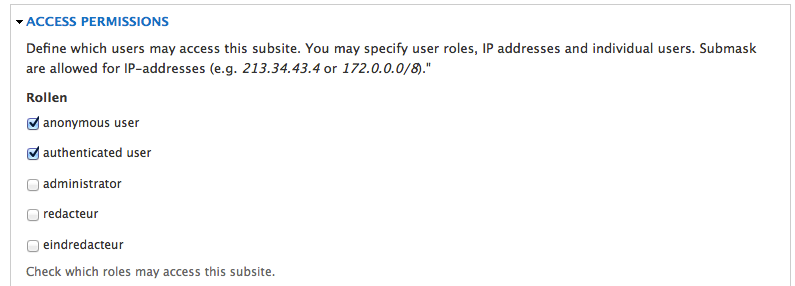
\includegraphics[width=\textwidth]{img/dominionaccess.png}
\end{center}

Hier kan worden aangevinkt welke gebruikersrollen toegang hebben tot deze subsite. Standaard staan "anonymous user" en "authenticated user" aan. Dit zijn respectieveliljk alle niet-ingelogde en alle ingelogde bezoekers en komt samen dus neer op alle bezoekers. Door deze uit te vinken en alleen de redacteurrollen aan te vinken zal deze subsite alleen toegankelijk worden voor redacteuren.





\section{Koppelingen}
In dit onderdeel wordt informatie gegeven over koppelingen naar andere systemen en koppelvlakken die andere systemen kunnen gebruiken om te integreren met \customerdomain .

\subsection{RSS}
\pvelist{ \pve{2.17}, \pve{2.17.1} }
De website biedt een aantal RSS feeds aan. Deze kunnen worden gebruikt om de laatste inhoud op te vragen in bijv. een RSS reader. De volgende feeds worden aangeboden:
\begin{itemize}
\item \drupalpath{nieuws/rss}: nieuwsberichten
\item \drupalpath{DOELGROEP/subsite/rss} doelgroep nieuwsberichten
\item \drupalpath{PROJECT/subsite/rss} project nieuwsberichten
\item \drupalpath{pers/persberichten/rss}: persberichten
\item \drupalpath{rss/documenten}: documenten
\item \drupalpath{rss/afbeeldingen}: afbeeldingen
\item \drupalpath{rss/bestanden/TAG}: bestanden per tag
\item \drupalpath{storingen/rss}: storingen
\item \drupalpath{werkzaamheden/rss}: werkzaamheden
\end{itemize}

\subsection{Twitter}
%todo PVE

Stap 1 in het hele proces is het registreren van een applicatie bij Twitter. Dit moet gebeuren voor alle omgevingen waarop de site draait (dus in het geval van ProRail op test, acceptatie en productie). Registratie verloopt via https://dev.twitter.com/apps/new

De callback URL is /twitter/oauth

In dit proces wordt een Consumer Key en Consumer Secret gegenereerd door Twitter. Deze zijn te vinden bij de Twitter applicatie.

Stap 2: Vul deze keys in op admin/settings/twitter
Stap 3: Koppel dit account \drupalpath{user/1/edit/twitter} door een nieuwe user toe te voegen.

De koppeling met Twitter wordt nu tot stand gebracht. Je ziet een inlogscherm van Twitter. Vul de inloggegevens in van het account waarvan je de tweets wilt toevoegen. Indien de inloggegevens goed zijn kom je terug op user/1/edit/twitter.
%todo screenshots
\subsection{Weer}
\pvelist{ \pve{4.18} }

\subsubsection{Weer alert}
De redacteur kan een weer alert plaatsen op de website door naar \drupalpath{admin/config/prorail/weather} te gaan en de \emph{Weather alert aanzetten} aan te vinken. Er verschijnt een blok op de homepage van ProRail en Reizigers. Er kan een titel en een tekst ingevuld worden die worden weergegeven in het blok. Ook wordt er een icoon geplaatst in het blok, dit icoon is het icoon van die dag die uit de data van Meteo Consult komt. Via de Lees meer link kan naar het weeroverzicht worden gegaan die ook beschikbaar is op de url \drupalpath{prorail/weersverwachtingen}.

\begin{center}
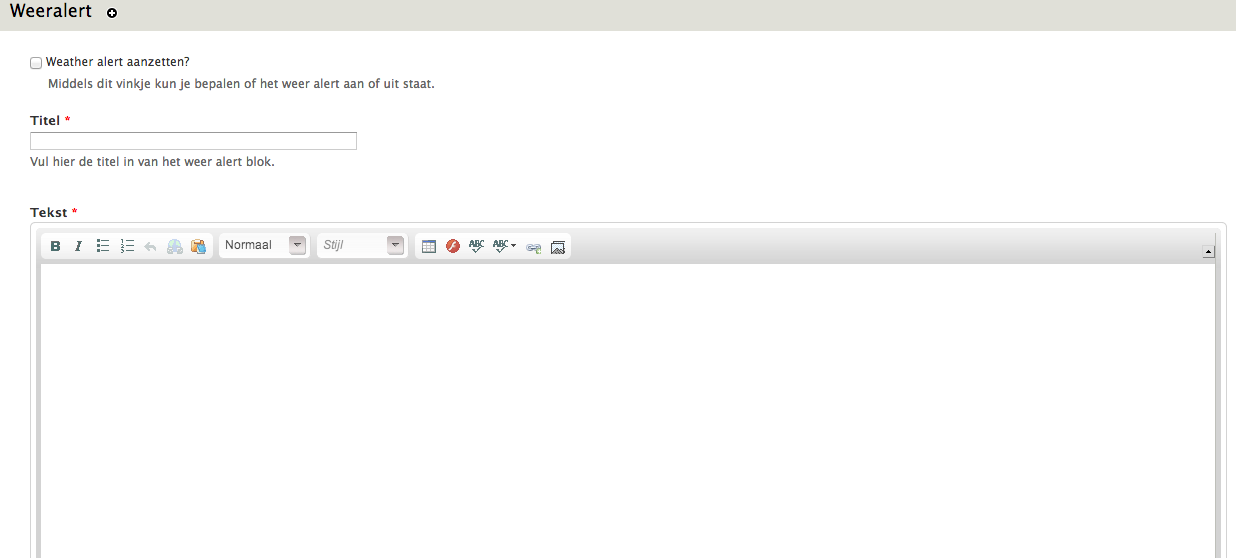
\includegraphics[width=\textwidth]{img/weeralert.png}
\end{center}

\subsubsection{Weer tekst}
De tekst bij de weersverwachting is te vinden bij het bewerken van die pagina in het "Intro" veld. Let erop dat de tekst niet in het bodyveld komt, want deze wordt overschreven door de import.

Tekst bij de kaart kan aangepast worden via de vertaalinterface: \drupalpath{/admin/config/regional/translate/translate}.
\subsection{Punctualiteit}

Blok kan via Felix toegevoegd worden en heet Punctualiteit. De content die in dat blok staat kan worden ingevuld op \drupalpath{/admin/config/prorail/punctualiteit} De volgende velden kunnen worden ingevuld:

\begin{enumerate}
\item Titel
\item Percentage
\item Percentage gemiddeld
\item Tekst
\item Link
\item Kleur (groen of rood voor Percentage veld)
\end{enumerate}


\subsection{Nieuwsbrief}
\pvelist{ \pve{4.25} }

De module ProRail Newsletter maakt gebruik van Drupal webforms voor het aanbieden 
van in- en uitschrijfformulieren voor nieuwsbrieven. Elke nieuwsbrief heeft 
\'{e}\'{e}n aanmeldformulier en \'{e}\'{e}n afmeldformulier. Aanmeldingen zijn 
eenvoudigweg inzendingen van de aanmeldformulieren. Er wordt niet voorzien in een 
koppeling naar een backendsysteem voor verzending, aanmeldingen dienen handmatig 
gedownload te worden als CSV-bestand (zie sectie \ref{sec:inzienaanmeldingen}). 
De module vult de webformulieren op twee belangrijke punten aan:

\begin{itemize}
\item Er wordt per aanmelding een uniek \emph{token} (een tekenreeks van 
willekeurige tekens) aangemaakt, dat meegestuurd moet worden in de 
bevestigingsemail (hiertoe moet de waarde van het tokenveld expliciet in de emailtemplate worden opgenomen) en er wordt in een bevestigingspagina voorzien, waarin 
het token verwerkt wordt en bij een juist token het veld \emph{Bevestigd} bij de aanmelding op 
\emph{Ja} wordt gezet (zie sectie \ref{sec:vereistenaanmeldformulieren}).
Op deze wijze is het niet mogelijk om een email-adres aan te melden via het 
formulier zonder toestemming van degene die werkelijk toegang heeft tot het 
email-adres. 
\item Bij het invullen van een afmeldingsformulier worden aanmeldingen voor het opgegeven 
email-adres (d.w.z. inzendingen van het bijbehorende aanmeldformulier) verwijderd.
\end{itemize}

\subsubsection{Standaard oplevering}
Bij oplevering is er als voorbeeld voorzien in twee aanmeldformulieren en een 
afmeldformulier. Het formulier \emph{Aanmelden nieuwsbrief} is ook daadwerkelijk 
geconfigureerd als aanmeldformulier, het formulier \emph{Aanmelden nieuwsbrief 
eenvoudig} is uitsluitend ter voorbeeld. Het afmeldformulier is gekoppeld aan 
het formulier \emph{Aanmelden nieuwsbrief}.
Afmeldingen kunnen, maar hoeven niet bekeken te worden; ze worden automatisch 
verwerkt, mits voldaan is aan de voorwaarden voor aan- en afmeldformulieren 
zoals hieronder opgesomd.  

\subsubsection{Inzien aanmeldingen}
\label{sec:inzienaanmeldingen}
Als voorbeeld bekijken we hoe de aanmeldingen voor de nieuwsbrief van het 
formulier \emph{Aanmelden nieuwsbrief} ingezien kunnen worden (dit is standaard webform-functionaliteit 
en werkt dus ook voor willekeurige andere webformulieren).

1. Zoek het formulier, bijvoorbeeld via de tab Webformulieren onder Inhoud
\begin{center}
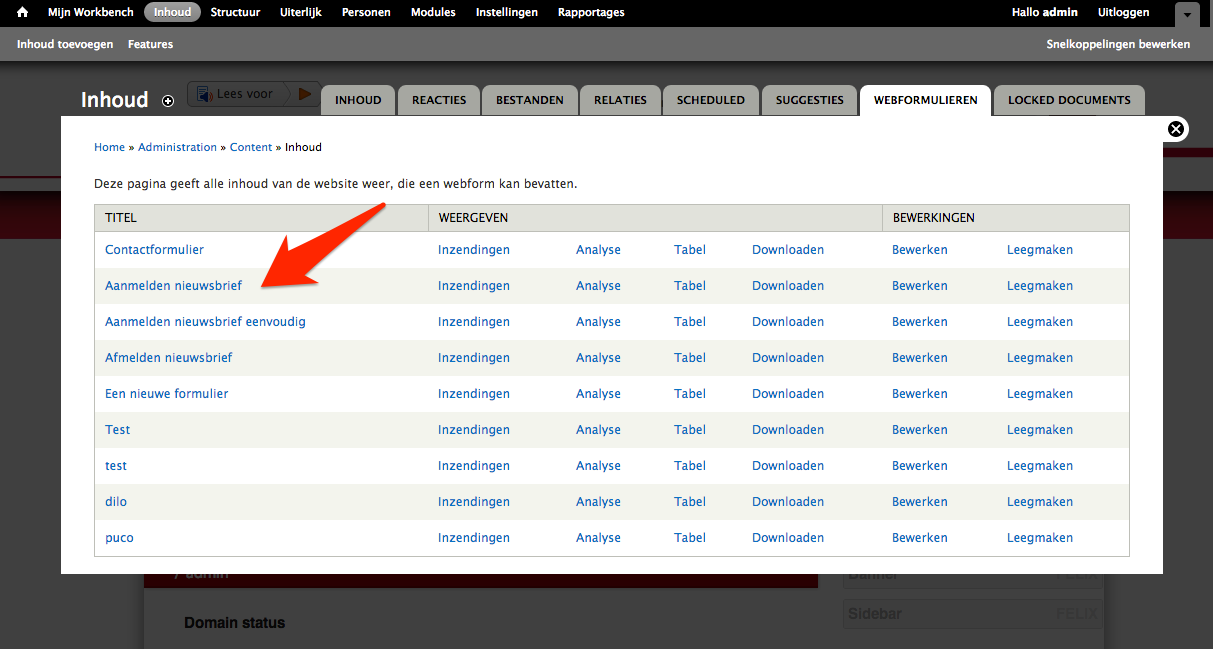
\includegraphics[width=\textwidth]{img/nieuwsbrief/form_aanmelden_nieuwsbrief.png}
\end{center}

2. Klik op de link Tabel
\begin{center}
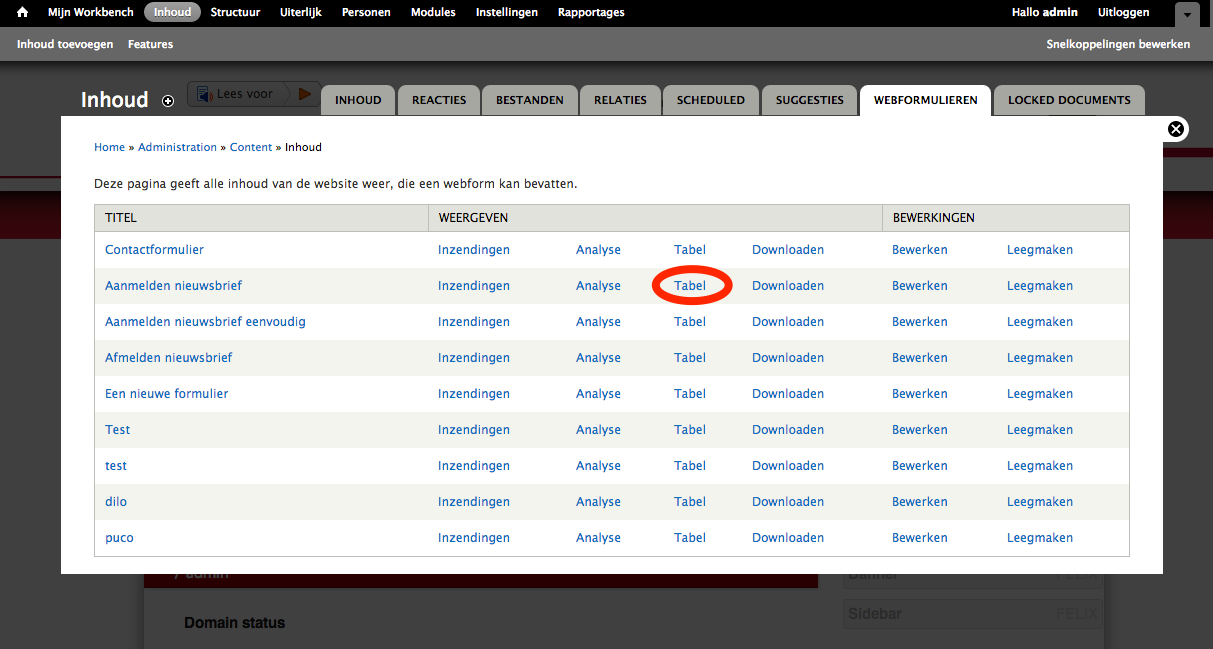
\includegraphics[width=\textwidth]{img/nieuwsbrief/aanmelden_nieuwsbrief_tabellink.png}
\end{center}

3. Een tabel met inzendingen verschijnt.
\begin{center}
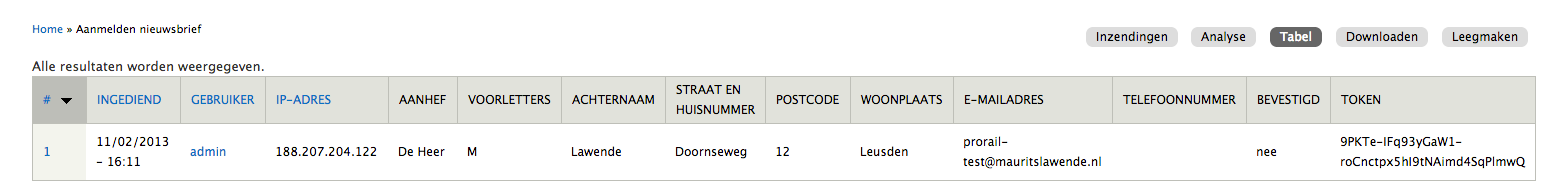
\includegraphics[width=\textwidth]{img/nieuwsbrief/aanmelden_nieuwsbrief_inzendingen.png}
\end{center}

4. De inzendingen kunnen gedownload worden als CSV-bestand op de link Download
\begin{center}
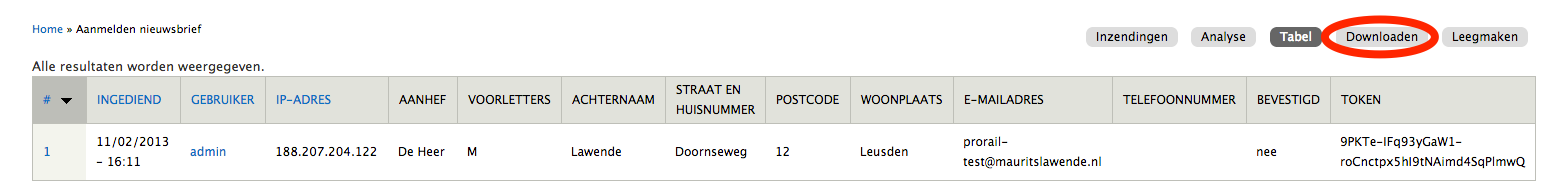
\includegraphics[width=\textwidth]{img/nieuwsbrief/aanmelden_nieuwsbrief_download.png}
\end{center}

Op dit scherm zijn een aantal instellingen mogelijk met bestrekking tot het te 
genereren export-bestand, zoals het scheidingsteken tussen waardes, welke waardes 
ge\"{e}xporteerd moeten worden en welke inzendingen gedownload moeten worden, zoals 
alleen nieuwe inzendingen, alle inzendingen, of een specifiek aantal inzendingen.

\textbf{Let op:} De download bevat alle aanmeldingen, inclusief de 
onbevestigde aanmeldingen. Het is dus bij verdere verwerking van het 
export-bestand van belang dat onbevestigde aanmeldingen worden uitgefilterd 
(dat zijn dus de aanmeldingen waarbij de kolom \emph{Bevestigd} niet op 
\emph{ja} staat).

N.b. Op het download-scherm kan gekozen worden voor het bestandsformaat 
\emph{Microsoft Excel}. Deze optie kan beter niet gebruikt worden, want de enige 
aanpassing die aan het gegenereerde bestand wordt gedaan is het veranderen van de 
bestandsnaamextensie in 
xls. De inhoud van het bestand blijft gelijk, waardoor het geen valide XLS-bestand is.

\subsubsection{Vereisten aanmeldformulieren}
\label{sec:vereistenaanmeldformulieren}
Aanmeldformulieren kunnen als normale webformulieren worden aangemaakt, mits ze aan 
een aantal eisen voldoen (op deze vereisten is geen actieve controle bij het selecteren 
van het formulier in de beheer-interface).

\begin{itemize}
\item Een veld met de machinenaam \emph{email}, dat het aangemelde email-adres bevat. Dit dient een veld van het type \emph{email} te zijn;
\item Een \emph{verborgen} veld met de machinenaam \emph{bevestigd}. Hiervoor moet 
de instelling \emph{veilige waarde} gebruikt worden zodat de 
waarde niet van buitenaf meegestuurd kan worden door middel van een malafide inzending. 
De standaard-waarde van dit veld moet op \emph{nee} ingesteld worden (in feite 
zijn hier geen beperkingen op anders dan dat de standaard-waarde niet \emph{ja}
mag zijn, want dat is de waarde die door de module wordt ingevuld bij bevestiging van 
de inschrijving).
\item Een \emph{verborgen} veld met de machinenaam \emph{token}. Dit veld wordt gebruikt voor het opslaan 
en controleren van het aangemaakte token. 
Ook hiervoor dient de instelling \emph{veilig waarde} gebruikt te worden. De 
standaard-waarde hoeft niet ingesteld te worden.
\item Een bevestigingsemail voor de gebruiker met daarin een bevestigingslink. De 
be\-ves\-ti\-gings\-link heeft de volgende vorm:
\url{http://www.prorail.nl/nieuwsbrief/bevestigen/\%value[token]}
Het voorbeeldformulier \emph{Aanmelden nieuwsbrief} bevat ook een voorbeeld van 
de bevestigingsemail met de token op de juiste manier erin opgenomen.
\end{itemize}

Naast deze velden kunnen eventueel andere velden naar keuze worden toegevoegd. Zo 
heeft het standaard opgeleverde aanmeldformulier velden voor postadres-gegevens. 
Aangeraden wordt om zo min mogelijk informatie van de gebruiker te vragen, zodat 
de drempel om voor een nieuwsbrief aan te melden zo laag mogelijk is.

\begin{figure}[p]
\centering
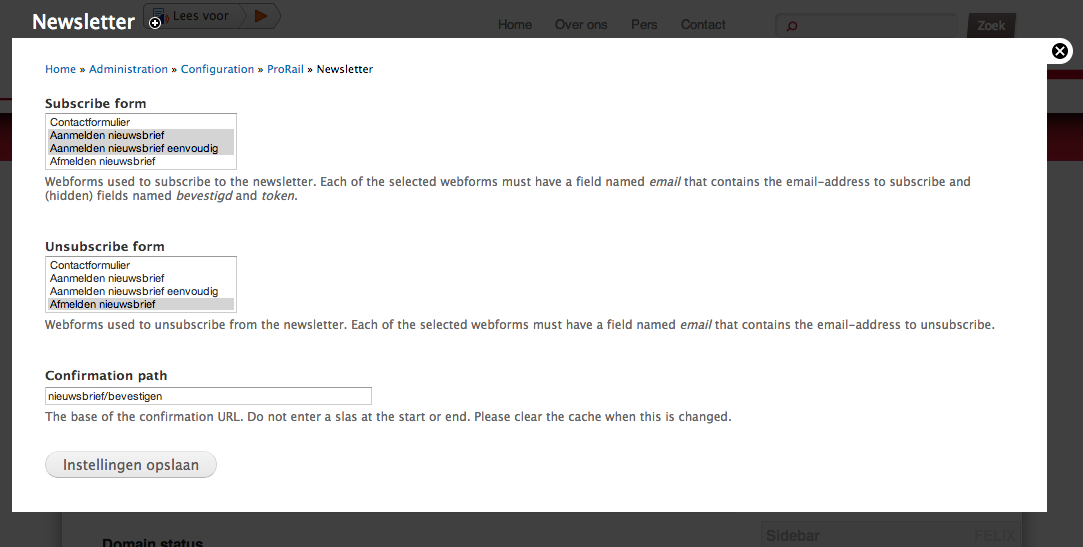
\includegraphics[width=\textwidth]{img/nieuwsbrief/nieuwsbrief_admin.png}
\end{figure}

\subsubsection{Vereisten afmeldformulieren}
\label{sec:vereistenafmeldformulieren}
De enige vereiste voor afmeldformulieren is dat ze een veld hebben met de 
machinenaam \emph{email} van het type \emph{email}. Extra velden kunnen naar 
eigen inzicht worden toegevoegd, bijvoorbeeld velden om een reden voor afmelding 
kenbaar te maken.

\subsubsection{Beheerinterface}
De beheer-interface van de module is te vinden onder Instellingen, ProRail, 
Newsletter.
De volgende instellingen zijn te maken:

\begin{itemize}
\item Het kiezen van webformulieren die dienst doen als aanmeldformulier (let op de vereisten 
zoals vermeld in \ref{sec:vereistenaanmeldformulieren}, of e.e.a. zal niet naar 
behoren werken).
\item Per aanmeldformulier een bijbehorend afmeldformulier (let op de vereisten 
zoals vermeld in \ref{sec:vereistenafmeldformulieren}).
\item Het instellen van het bevestigings-pad, dat wil zeggen de URL die de 
bevestigingen dient te verwerken. Dit is de link die vermeld dient te worden in de 
bevestigingsemail, die verantwoordelijk is voor het verwerken van aanmeldingstokens. 
Normaal gesproken hoeft dit niet aangepast te worden.
\end{itemize}

\subsubsection{Settings}

De module is instelbaar op admin/config/prorail/newsletter. Hier zijn de volgende zaken in te stellen:

\begin{enumerate}
\item Welke formulieren gelden als inschrijfformulier. Deze formulieren dienen een veld voor het email-adres te hebben met als sleutelveld 'email' en een tweetal verborgen velden, met de keys 'bevestigd' en 'token'. 'token' wordt bij indienen gevult met een unieke string, die in de bevestigingsemail wordt opgenomen in een link waarmee de aanmelding bevestigd moet worden (zie verder). 'bevestigd' wordt op 'ja' gezet zodra deze link bezocht is.

\item Welke formulieren gelden als afmeldformulier. Een email-adres ingevuld in het formulier-element met de sleutelveld 'email' heeft tot gevolg dat inzendingen van de aanmeldformulieren met dat email-adres worden verwijderd.

\item De basis voor bevestigings-URLs. Hier wordt het aangemaakte token aan vastgeplakt. Bijvoorbeeld: "nieuwsbrief/bevestigen". Het is van belang dat de URL die in de email wordt gezet hiermee overeenkomt. (Indien dit wordt verandert moet de cache gelegd worden omdat de menu router-tabel opnieuw opgebouwd moet worden).
\end{enumerate}

Voor de bevestigingsemail wordt de normale Webforms email-voorziening gebruikt. De bevestigingstoken is daar beschikbaar als value[token]. Dit is voor de huidige aanmeldformulieren al juist ingesteld.

\subsubsection{Formulieren nieuwsbrieven}

Een ingelogde gebruiker kan het formulier invullen. Er wordt dan geen e-mail verstuurd. Wel zie je de confirmatiepagina die reguliere gebruikers ook zien, waar staat dat er een e-mail is verstuurd (let dus op: dit gebeurt niet als je als content beheerder het formulier hebt ingevuld.).

Als ingelogde gebruiker kun je ook verplichte velden overslaan.

\begin{figure}[p]
\centering
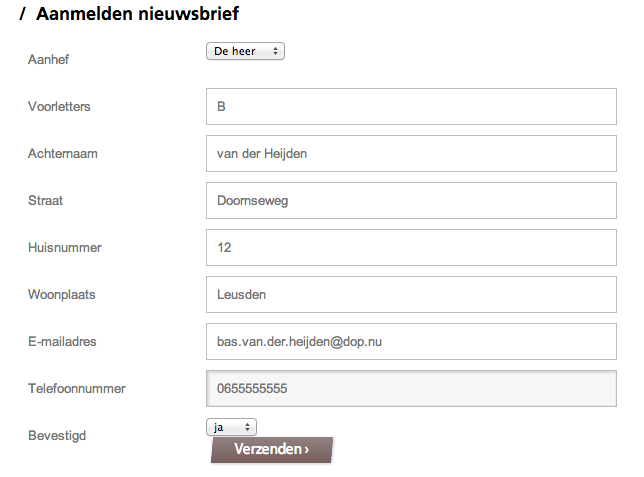
\includegraphics[width=\textwidth]{img/nieuwsbrief/nieuwsbrief_formulier.png}
\end{figure}


\subsection{CRM}

De koppeling naar het CRM is gebaseerd op de standaard Drupal formulieren\see{webform}. Hiermee zijn twee formulieren ingericht:
\begin{itemize}
\item Publiekscontacten
\item Aanvragen applicaties (digitaal loket)
\end{itemize}
Deze formulieren zijn in beperkte mate aanpasbaar via het CMS. Wijzigingen kunnen worden doorgevoerd, maar de velden dienen te corresponderen met de velden die aangemaakt zijn in het CRM pakket. Bij het bewerken en toevoegen van de node is een veld zichtbaar met label "CRM entiteit". Dit is de technische naam waaronder inzendingen worden opgeslagen. Dit veld is niet verplicht. Bij geen invoer wordt het formulier niet aan CRM gekoppeld.

Onder het tabblad "Webform" kunnen de velden worden ingesteld\see{webform}. De velden hebben een technische naam ("sleutelveld") die exact overeen moet komen met de naam in CRM. Velden die niet overeenkomen zullen niet in CRM terecht komen. Onder het tabblad "CRM fields" is een overzicht te zien van de velden die beschikbaar zijn in de gekozen entiteit. Velden worden rood getoont indien er geen veld gekoppeld is. De velden die groen zijn gekleurd zullen wel in CRM terechtkomen.

De lijsten van beschikbare entiteiten en velden in CRM zijn afkomstig uit de WSDL en verwerkt in de Drupal module. Bij wijzigingen (nieuwe velden / entiteiten) in het CRM systeem zelf zal de module ook aangepast moeten worden. Dat proces gaat niet automatisch, maar het is wel mogelijk om via bovenstaande werkwijze nieuwe formulieren te maken die koppelen met bestaande entiteiten / velden.



\clearpage

\appendix
%\appendixpage\label{appendices}
\addappheadtotoc

%\index{PvE}{shizzle|none}
\printindex{pve}{PvE}

%\index{Paden}{shizzle|none}
\printindex{drupalpath}{Paden}


%\section{Modulereferentie}\label{tools}

\begin{multicols}{2}
%\printindex{modules} werkt niet.
%\input{modules.ind}
\end{multicols}

%\include{parts/appendices/imagecache-presets} % Eerste appendix-pagina is alleen een titeltje, dus doorgaan op dezelfde pagina met \input ipv \include.


\end{document}
